\documentclass[english, 12 pt]{report}
\usepackage[T1]{fontenc}
\usepackage[utf8]{luainputenc}
\usepackage{lmodern} % load a font with all the characters
\usepackage{babel}
\usepackage[hidelinks, bookmarks]{hyperref}
\usepackage{geometry}
\geometry{verbose,tmargin=1cm,bmargin=3cm,lmargin=4cm,rmargin=4cm,headheight=3cm,headsep=1cm,footskip=1cm}
\setlength{\parindent}{0bp}
\usepackage{amsmath}
\usepackage{amssymb}
\usepackage{esint}
\usepackage{import}

\usepackage{graphicx}
\usepackage{placeins}
\raggedbottom
\usepackage{calc}
\usepackage{cancel}
\makeatletter
\usepackage{color}
\definecolor{shadecolor}{rgb}{0.105469, 0.613281, 1}
\usepackage{framed}
\usepackage{wrapfig}
\usepackage{bm}
\usepackage{ntheorem}
\usepackage{ragged2e}
\RaggedRight
%\raggedbottom
\frenchspacing
\newcommand{\vsk}{\newline\vspace{11 pt}}
\newcommand\alg[1]{\begin{align*} #1 \end{align*}}
\pagenumbering{gobble}
\begin{document}
\textsl{De grønne trekantene på bildet er like store. Dei oransje rektangla er også like store.}
\begin{enumerate}
	\item Klipp ut det raude kvadradet, dei oransje rektangla, det rosa kvadratet, det blå kvadratet og dei grøne trekantane fra figurane uten tal og bokstavar på. (Det er viktig at du klipper fint).
	\item Er det ein samanheng mellom nokon av formene som er klipt ut?
	\item Sett figurane saman slik dei var før klippinga. Om ein tek vekk dei oransje rektangla, kor mange grøne trekantar må ein ta vekk for at figurane skal ha same areal?
	\item Hva er sammanhengen mellom det raude, det rosa og det blå kvadratet?
	\item Sjå på figurene med tall på. Kva er verdien til $ c $?
	\item Sjå på figurene med bokstaver på. Kva er uttrykket for arealet til \textsl{a)} det raude kvadratet? \textsl{b)} det lilla kvadratet? \textsl{c)} det blå kvadratet?
	\item Kva er samanhengen mellom uttrykka du fann i oppgåve 6?
	\item Diskuter: Viss ein trekant er rettvinkla, vil ein alltid kunne lage ein figur som denne?
		\begin{figure}[hbt]
		\centering
		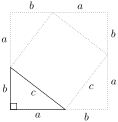
\includegraphics[]{pyt}
	\end{figure}
	\item Kva er Pytagoras' setning?
			\begin{figure}[hbt]
		\centering
		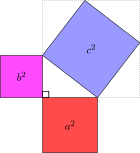
\includegraphics[]{pyb}
	\end{figure}
\end{enumerate}

\newpage
\begin{figure}[hbt]
	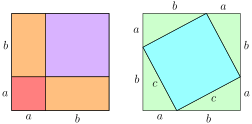
\includegraphics[]{tri26d}
\end{figure}

\end{document}